\section{Introduction}
\label{sec:intro}
The present work targets the problem of segmenting medical sequences using sparse point-wise supervision.
An annotator is given a video or volume that contains a single object of interest, and is asked to give a maximum of one click on each frame where the object lies.
In \cite{lejeune18}, authors provide a general framework that builds up on multi-object tracking.
In particular, the segmentation problem is formulated as a maximum a posteriori problem where the binary random variable to optimize for assign superpixels to the foreground or background.
Through the Markov assumption, the problem is then cast into a network flow problem.
The latter approach requires two kind of models to determine the costs associated to edges.
(1) A foreground model, which gives the cost that a path would incur when transiting through a given superpixel, and (2) and transition model which gives the cost of passing from one superpixel to another located on a past or future frame.

Despite the effectiveness of the latter approach, we note that component (1) requires to train an auto-encoder as a pretext task to obtain deep-features, which are then used by a simple bagging of decision trees applicable to PU learning to infer the foreground probabilities.
First, as the late-stage bagging model considers all over-segmented regions as independent samples,
the spatial configuration of the object of interest is not explicitly taken into account.
Second, even though authors add an image-wise gaussian prior to the reconstruction error as an attempt to penalize errors around the object of interest,
the loss function of the auto-encoder does not specifically target the task of segmentation.

In the present work, we overcome the above limitations through the following contributions.
\begin{itemize}
    \item We take a more direct approach by leveraging the non-negative unbiased risk estimator of \cite{kiryo17}, which we use as a loss function of a Convolutional Neural Network to infer the foreground probabilities.
  \item Furthermore, as the latter loss function requires accurate class-priors to be effective,
    we devise a self-supervised strategy to estimate them through a recursive bayesian approach, initialized with a single upper-bound value.
\end{itemize}

\begin{figure*}[t]
\centering
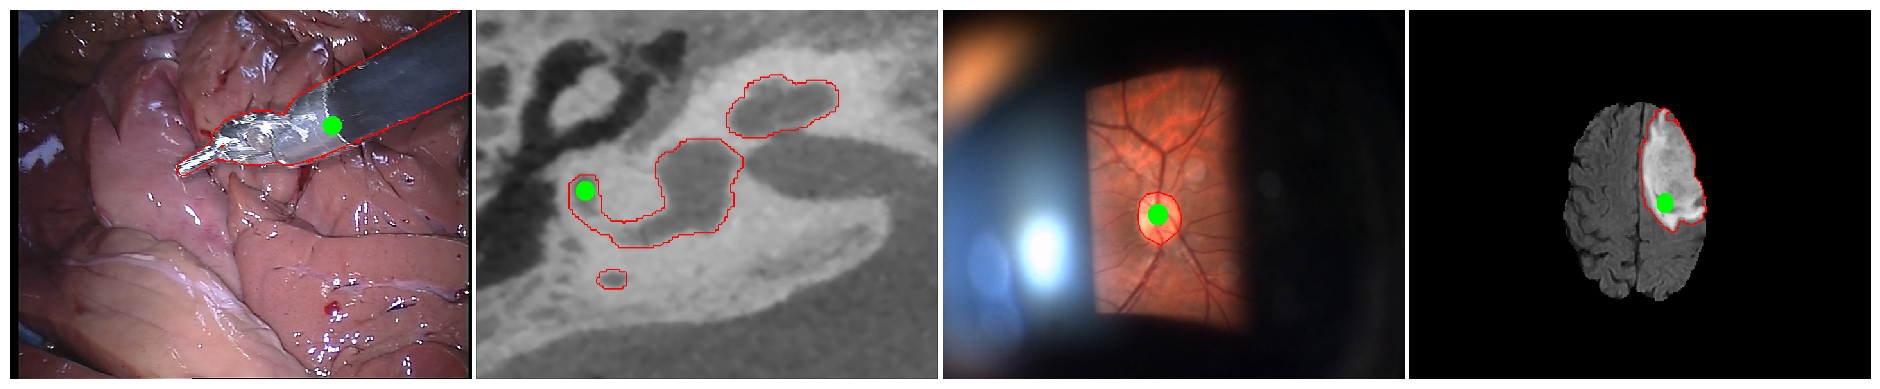
\includegraphics[width=0.9\textwidth]{pics/intro.png}
\caption{For each sequence, we show an example frame with user-provided 2D location in green and groundtruth in red. From left to right: Tweezer, Cochlea, Slitlamp, Brain}
\label{fig:intro}
\end{figure*}


%%% Local Variables:
%%% mode: latex
%%% TeX-master: "../../main"
%%% End:
